\documentclass[12pt]{article}

\usepackage{fontspec}
\usepackage{polyglossia}
\usepackage{geometry}
\usepackage{graphicx}

\usepackage{amsmath,
            amsthm,
            amssymb
}

\usepackage{unicode-math,
            tensor
}

\usepackage{wrapfig, 
            hyperref,
            multicol,
            multirow,
            tabularx,
            booktabs,
            makecell
}

\usepackage{}

\geometry{a4paper,
          total={170mm,255mm},
          left=10mm,
          top=15mm,
}

\setdefaultlanguage{russian}
\setotherlanguage{english}
\setkeys{russian}{babelshorthands=true}

\defaultfontfeatures{Ligatures=TeX}
\setmainfont{STIX Two Text}
\setmathfont{STIX Two Math}
\DeclareSymbolFont{letters}{\encodingdefault}{\rmdefault}{m}{it}

\newfontfamily{\cyrillicfont}{STIX Two Text} 
\newfontfamily{\cyrillicfontrm}{STIX Two Text}
\newfontfamily{\cyrillicfonttt}{Courier New}
\newfontfamily{\cyrillicfontsf}{STIX Two Text}

\renewcommand{\thefigure}{\thesection.\arabic{figure}}
\renewcommand{\thetable}{\thesection.\arabic{table}}
\numberwithin{equation}{section}

\renewcommand{\qedsymbol}{$\blacksquare$}
\theoremstyle{definition}
\newtheorem{definition}{Опр.}[section]
\theoremstyle{remark}
\newtheorem{statement}{Утв.}[section]
\theoremstyle{plain}
\newtheorem{theorem}{Теор.}[section]

\addto\captionsrussian{
  \renewcommand{\figurename}{Рис.}
  \renewcommand{\tablename}{Табл.}
  \renewcommand{\proofname}{Док-во}
}

\graphicspath{{./img/}}
\everymath{\displaystyle}

\newcommand{\RNumb}[1]{\uppercase\expandafter{\romannumeral#1\relax}}
\newcommand{\llabel}[1]{\label{\thesubsection:#1}}
\newcommand{\lref}[1]{\ref{\thesubsection:#1}}

\begin{document}
\paragraph{О-07}
Дифракционная решетка. Основная формула. Главные и второстепенные максимумы. Ширина $m$-го главного максимума. Спектр $n$-го порядка. Угловая дисперсия, критерий Рэлея, разрешающая способность.\\

Дифракционная решетка представляет собой простой спектральный прибор, т.е. прибор, позволяющий исследовать спектральный состав света. Она позволяет различать компоненты, которые для глаза кажутся одного цвета.
Дифракция Фраунгофера – дифракция в параллельных лучах, и поэтому она обладает важным свойством: дифракционные картины от двух смещенных друг относительно друга объектов накладываются друг на друга без смещения. Именно это свойство используется в дифракционной решетке, представляющей собой большое количество $N$ одинаковых щелей, расстояние между которыми постоянно. Расстояние  $d$  между серединами соседних щелей называется периодом решетки. Ширину щели, как и раньше, будем обозначать буквой $b$.

\begin{figure}[h]
\begin{center}
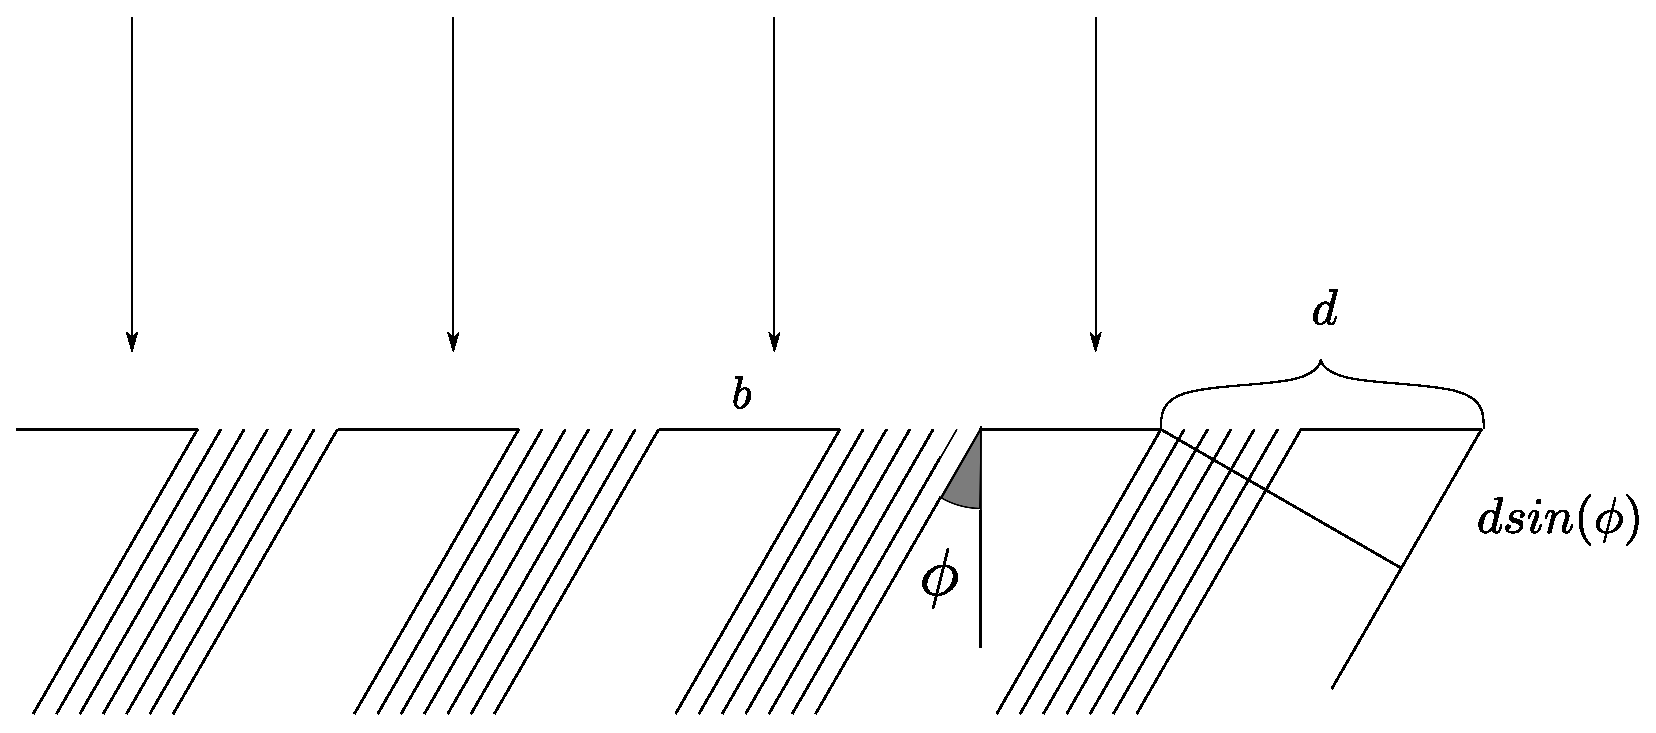
\includegraphics[width=0.5\linewidth]{img/o-07_1.eps}
\caption{Дифракционная решетка}
\end{center}
\end{figure}

Пусть $E^{(1)} (\varphi)$ - световое поле, посылаемое одной щелью под углом $\phi$ к нормали. Тогда поле от $N$ записывается как суперпозиция:
$$E^{(N)}(\varphi) = E^{(1)}(\varphi)(1 + e^{ik\Delta} + ... + e^{ik(N-1)\Delta}),$$
где $\Delta = d\sin \varphi$ - оптическая разность хода между лучами, идущими от соседних щелей. Слагаемые в скобке образуют геометрическую прогрессию с суммой:
$$\frac{1-e^{iNk\Delta}}{1-e^{ik\Delta}} = \frac{e^{iNk\frac{\Delta}{2}}}{e^{ik\frac{\Delta}{2}}}\cdot \frac{e^{iNk\frac{\Delta}{2}} - e^{-iNk\frac{\Delta}{2}}}{e^{ik\frac{\Delta}{2}} - e^{-ik\frac{\Delta}{2}}},$$
Введем для удобства переменную $\delta = \frac{kd\sin\varphi}{2}$, получаем:
$$E^{(N)}(\varphi) = E^{(1)}(\varphi)\frac{e^{iN\delta}}{e^{i\delta}}\cdot \frac{\sin N\delta}{\sin\delta}$$
Для интенсивности:
$$I^{(N)}(\varphi) = I^{(1)}(\varphi)\frac{\sin^2 N\delta}{\sin^2\delta}$$
Если $\sin \delta$ в знаменателе дает 0, то и числитель равен 0. это случается, когда $\delta = m\pi \rightarrow kd\sin\varphi = 2m\pi$. Получаем условие для главного максимума:
$$d\sin(\varphi^{max}_m) = m\lambda,$$
где $m = 0, \pm 1, \pm 2...$ - порядок главного максимума. Интенсивность в главном максимуме очень велика. Поскольку синус меньше единицы, число наблюдаемых главных максимумов удовлетворяет условию:
$$m < \frac{d}{\lambda}$$
Числитель дроби в формуле для интенсивности также может обращаться в 0 при $N\delta = p'\pi, $ но $\delta \neq m\pi$, $p' = \pm 1, p\pm 2, ...$, т.е. когда $d\sin(\varphi ^{min}_{p'} = \frac{p'}{N}\lambda, \frac{p'}{N} \neq m$  
Это минимумы с нулевой интенсивностью, условия можно записать в более удобном виде. Если $p' = 0, $ то $m = 0$ и это максимум нулевого порядка. Далее годятся все $p' = \pm1, \pm2, ... , \pm(N-1). $ При $p' = \pm N$ получаются симметричные главные максимумы первого порядка. Далее отношение $\frac{p'}{N}$ можно записать как $1 + \frac{p}{N}, p =  \pm1, \pm2, ... , \pm(N-1)$. Далее появляются максимумы второго порядка. Продолжая это рассмотрение, приходим к условию минимумов:
$$d \sin(\varphi^{min}_{m, p}) = (m + \frac{p}{N})\lambda$$
Мы видим, что между ближайшими друг к другу максимумами находится $N - 1$ минимумов. Ясно, что минимумы отделены друг от друга максимумами, и если это не главные максимумы, то они называются второстепенными или побочными. В частности, для ближайших к $m$-му главному максимуму минимумов:
$$d\sin(\varphi^{min}_{m, \pm1} = (m \pm \frac{1}{N})\lambda$$
Найдем угловую ширину главного масимума $\delta\varphi$ как угловое расстояние между ближайшими к нему минимумами:
$$\delta\varphi = \varphi^{min}_{m, 1} - \varphi^{min}_{m, -1} $$
Ясно, что 
$$\varphi^{min}_{m, -1} = \varphi^{max}_{m} - \frac{\delta \varphi}{2}$$
$$\varphi^{min}_{m, 1} = \varphi^{max}_{m} + \frac{\delta\varphi}{2}$$
$$d(\sin(\varphi^{max}_{m} + \frac{\delta\varphi}{2}) - \sin(\varphi^{max}_{m} - \frac{\delta\varphi}{2})) = \frac{2\lambda}{N} $$
$$d\sin(\frac{\delta \varphi}{2} \cos(\varphi^{max}_m) = \frac{\lambda}{N}$$
$$\delta\varphi << 1 \rightarrow \sin(\frac{\delta\varphi}{2} \approx \frac{\delta\varphi}{2}$$
Для угловой ширины максимума получается следующая формула:
$$\delta\varphi = \frac{2\lambda}{dNcos(\varphi^{max}_m)}$$
Cпектр $n$-го порядка - по сути, второстепенные максимумы (радужки), расположенные между главными максимумами N и N+1 порядков.\\
Основная задача использования спектральных приборов – различить близкие по длине волны линии ($\delta \lambda = \lambda_2 - \lambda_1$) спектра излучения. Для этого, прежде всего, нужно, чтобы главные максимумы таких линий были достаточно разнесены по углу, поэтому вводится такая спектральная характеристика прибора как угловая дисперсия – отношение разности углов $\delta\varphi$, под которыми видны две линии к разности длин волн излучения $\delta\lambda$:
$$D_\varphi = \frac{\delta\varphi}{\delta\lambda}$$
Для решетки эта характеристика находится очень просто – взятием дифференциала от левой и правой частей условия для главных максимумов (будем писать просто $\varphi$ вместо $\varphi^{max}_m$)
\begin{gather*}
d\cos\varphi \delta\varphi = m\delta\lambda\\
D_\varphi = \frac{m}{d\cos \varphi}
\end{gather*}
Критерий Рэлея: две линии находятся на пределе разрешения, если максимум одной из них приходится на границу другой.\\
Разрешающей способностью называется величина
$$R = \frac{\lambda}{\delta\lambda_{min}},$$
где $\delta\lambda_{min}$ - минимальная разность двух длин волн, линии которых оказываются разрешенными этой решеткой. \\
Найдем выражение для разрешающей способности решетки при использовании критерия Рэлея. Пусть максимум линии для волны $\lambda' = \lambda + \delta\lambda_{min}$ совпадает с минимумом линии $\lambda$ под углом $\varphi$
Тогда:
\begin{gather*}
d\sin\varphi = m(\lambda + \delta \lambda_{min})\\
d\sin\varphi = (m + \frac{1}{N})\lambda\\
m\delta\lambda_{min} = \frac{\lambda}{N} \longrightarrow R = mN
\end{gather*}
\end{document} 
